% \documentclass[a4paper,10pt]{article}
\documentclass[review]{siamart}
\usepackage{url}
\usepackage{amssymb}
\usepackage{amsmath}
\usepackage{bm}
\usepackage{stmaryrd}
\usepackage{array}
\usepackage{empheq}
\usepackage{enumitem}
	\setlist{nosep} % or \setlist{noitemsep} to leave space around whole list
\usepackage{color}
%\usepackage{showlabels}
\usepackage{adjustbox}
\usepackage{hyperref}
\hypersetup{
  colorlinks   = true, %Colours links instead of ugly boxes
  urlcolor     = blue, %Colour for external hyperlinks
  linkcolor    = blue, %Colour of internal links
  citecolor   = red %Colour of citations
}
\usepackage[numbers,sort]{natbib}
\usepackage{cleveref}

\newsiamremark{remark}{Remark}


% \newtheorem{lemma}{Lemma}
% \newtheorem{definition}{Definition}
% \newtheorem{theorem}{Theorem}
% \newtheorem{corollary}{Corollary}

\newcommand{\rc}{\textcolor{red}{,}}

\newcommand{\tcb}{\textcolor{blue}}
\newcommand{\tcp}{\textcolor{purple}}
\newcommand{\todo}[1]{\textcolor{red}{[TODO\@: #1]}}

\newcommand{\mdet}{\operatorname{det}}
\newcommand{\madj}{\operatorname{adj}}

% ------------------------------------------------------------------------------------ %
% ------------------------------------------------------------------------------------ %

\newcommand{\TheTitle}{IRK!}
\newcommand{\TheAuthors}{B.S. Southworth }
\headers{IRK!}{\TheAuthors}
\title{{\TheTitle}\thanks{This research was conducted ...
  }}

\author{%
  Ben~S.~Southworth
  \thanks{Department of Applied Mathematics,
          University of Colorado at Boulder
          (\email{ben.s.southworth@gmail.com}).}
}

\ifpdf%
\hypersetup{%
  pdftitle={\TheTitle},
  pdfauthor={\TheAuthors}
}
\fi

% ------------------------------------------------------------------------------------ %
% ------------------------------------------------------------------------------------ %

\begin{document}
\allowdisplaybreaks


% ------------------------------------------------------------------------------------ %
% ------------------------------------------------------------------------------------ %
% ------------------------------------------------------------------------------------ 
\newpage
\newpage
\section{Nonlinear}
Have ODEs,
%
\begin{align}
	M\mathbf{u}'(t) =  \mathcal{N}(\mathbf{u},t) \quad\text{in }(0,T], \quad \mathbf{u}(0) = \mathbf{u}_0,
\end{align}
%
where $M$ is a mass matrix and $\mathcal{N} \colon \mathbb{R}^{N} \times \mathbb{R}_+ \to \mathbb{R}^{N}$ is a discrete, time-dependent, nonlinear operator. Then, an $s$-stage IRK scheme approximately propagates the discrete  solution by
%
\begin{align}
\mathbf{u}_{n+1} & = \mathbf{u}_n + \delta t \sum_{i=1}^s b_i\mathbf{k}_i,
\end{align}
with stage vectors satisfying the block system of $s$ nonlinear equations,
\begin{align}
M\mathbf{k}_i & = \mathcal{N}\left(\mathbf{u}_n + \delta t\sum_{j=1}^s a_{ij}\mathbf{k}_j, t_n+\delta tc_i\right), \quad i = (1,\ldots,s).
\end{align}

For a given pair $(\bm{u}_n,t_n)$, let's define the operator $F_i \colon \mathbb{R}^{sN} \to \mathbb{R}^N$ that encodes the $i$th stage vector,
\begin{align}
F_i(\bm{k}) \coloneqq M \bm{k}_i - {\cal N} \left(\bm{u}_n + \delta t \sum \limits_{j = 1}^s a_{ij} \bm{k}_j, t_n + c_i  \delta t \right),
\end{align}
with $\bm{k} = (\bm{k}_1, \ldots, \bm{k}_s)^\top$ the vector of stages. Then, the nonlinear system we need to solve to advance forwards one time step is
\begin{align}
\begin{bmatrix}
F_{1}(\bm{k})\\
\vdots \\
F_{s}(\bm{k})
\end{bmatrix}
\eqqcolon F(\bm{k}) = 0.
\end{align}
%
%Let's say we solve this system via a Newton-type method. That is, we apply a fixed-point algorithm like 
%\begin{itemize}
%\item Given initial iterate $\bm{\hat{k}} \approx \bm{k}$, if $\Vert F(\bm{\hat{k}}) \Vert > \varepsilon$, 
%\item Solve $G(\bm{\hat{k}}) \bm{d} = - F(\bm{\hat{k}})$, where $G(\bm{x}) \approx F'(\bm{x})$ is some approximation of the Jacobian of $F$ evaluated at $\bm{x}$
%\item Update iterate $\bm{\hat{k}} \to \bm{\hat{k}} + \bm{d}$ 
%\item If $\Vert F(\bm{\hat{k}}) \Vert > \varepsilon$, repeat
%\end{itemize}
%
%The particular method will be defined by the approximate Jacobian, $G$. Note the true Jacobian matrix is
%\begin{align}
%F'(\bm{\hat{k}}) = 
%\begin{bmatrix} M \\ 
%& \ddots \\ 
%& & M
%\end{bmatrix}
%- 
%\delta t
%\begin{bmatrix} {\cal L}_1 \\ 
%& \ddots \\ 
%& & {\cal L}_s
%\end{bmatrix}
%(A_0 \otimes I)
%\end{align}
%where
%\begin{align}
%{\cal L}_i \coloneqq {\cal N}' \left(\bm{u}_n + \delta t \sum \limits_{j=1}^s a_{ij} \bm{\hat{k}}_j, t_n + c_i \delta t \right).
%\end{align}
%
%In the formulation, we factor out a part of the Schur decomposition of $A_0 = Q_0 R_0 Q_0^\top$, and, so the linear systems we actually solve during a Newton-like step take the form
%\begin{align}
%\big[ R_0 \otimes M - (Q_0^\top \otimes  I) L (Q_0 \otimes I) \big] 
%(R_0^{-1} Q_0^\top \otimes I) \bm{d} = - (Q_0^\top \otimes I) F( \bm{k}^0).
%\end{align}
%where $L \approx {\rm diag}({\cal L}_1, \ldots, {\cal L}_s)$.
%
%During each Newton iteration, we first solve the system
%\begin{align}
%\big[ R_0 \otimes M - (Q_0^\top \otimes  I) L (Q_0 \otimes I) \big]  \bm{z} = \bm{y}
%\end{align}
%via backward substitution, where $ \bm{y} = - (Q_0^\top \otimes I) F( \bm{k}^0)$. Then we solve for $\bm{d} = (Q_0 R_0 \otimes I) \bm{z}$ via simple multiplication.



\tcp{But rather than solving this nonlinear system, we make a slight change of variables.}
Say we make the following simple change of variables:
\begin{align}
\bm{w} = (A_0 \otimes I) \bm{k} 
\quad 
\Longleftrightarrow 
\quad
\bm{k} = (A_0^{-1} \otimes I) \bm{w}
\end{align}
and we first solve the nonlinear problem for $\bm{w}$, then solve a linear problem to obtain $\bm{k}$ from $\bm{w}$ (well, we'd actually obtain $(\bm{b}_0^\top \otimes I) \bm{k} = (\bm{b}_0^\top A_0^{-1} \otimes I) \bm{w} = (\bm{d}_0^\top \otimes I) \bm{w}$ since this is what we really need). Now the nonlinear system becomes
\begin{align}
F(\bm{w}) = ( A_0^{-1} \otimes M ) \bm{w} - 
\begin{bmatrix}
{\cal N}(\bm{u}_{n} + \delta t \bm{w}_1, t_n + c_1 \delta t)\\
\vdots\\
{\cal N}(\bm{u}_{n} + \delta t \bm{w}_s, t_n + c_s \delta t)\\
\end{bmatrix}
= 
0.
\end{align}

\begin{remark}[Nonlinear decoupling]
What's interesting here is that the components of $\bm{w}$ are now only linearly coupled to each other (via the $A_0^{-1} \otimes M$ term), where with the previous formulation the components of $\bm{k}$ were nonlinearly coupled (every equation involves ${\cal N}$ being evaluated with $(\bm{k}_i)_{i =1}^s$). 
This may be useful for a Picard iteration or something, since now the $s$ systems can maybe be solved in parallel. 
\end{remark}

The Jacobian is
\begin{align}
F'(\bm{w}) = A_0^{-1} \otimes M - 
\delta t
\begin{bmatrix} {\cal N}'_1 \\ 
& \ddots \\ 
& & {\cal N}'_s
\end{bmatrix}
\end{align}
where
\begin{align}
{\cal N}'_i \equiv {\cal N}' \left(\bm{u}_n + \delta t \bm{w}_i^0, t_n + c_i \delta t \right).
\end{align}

The linear systems we solve during the Newton-like solve take the form
\begin{align}
\big[ R_0 \otimes M - (Q_0^\top \otimes  I) (\delta t N')  (Q_0 \otimes I) \big] 
(Q_0^\top \otimes I) \bm{ \delta w } = - (Q_0^\top \otimes I) F( \bm{w}),
\end{align}
by using the Schur decomposition of $A^{-1}_0 = Q_0  R_0 Q^{\top}_0$ with block upper triangular $R_0$. And, 
\begin{align}
N' \approx  
\begin{bmatrix} {\cal N}'_1 \\ 
& \ddots \\ 
& & {\cal N}'_s
\end{bmatrix}.
\end{align}

\subsection{A simplified Newton}
We take
\begin{align}
N' = 
\begin{bmatrix} {\cal N}'_s \\ 
& \ddots \\ 
& & {\cal N}'_s
\end{bmatrix}
= 
I \otimes {\cal N}'_s,
\end{align}
such that the matrix 
\[\big[ R_0 \otimes M - (Q_0^\top \otimes  I) (\delta t N')  (Q_0 \otimes I) \big] = 
\big[ R_0 \otimes M - \delta t N' \big] \] is block upper triangular, and can be inverted via backward substitution. During this solve, we have to invert the diagonal blocks, which take the form
\begin{align}
1 \times 1 \textrm{ systems:} \quad \zeta_j M - \delta t {\cal N}'_s,
\end{align}
and 
\begin{align}
2 \times 2 \textrm{ systems:} \quad
\begin{bmatrix}
\eta_j M  - \delta t {\cal N}'_s & \phi M \\
-\tfrac{\beta^2_j}{\phi} M & \eta_j M  - \delta t {\cal N}'_s \\
\end{bmatrix}
\end{align}

This is done with preconditioned GMRES, where for the $1 \times 1$ system, a single AMG iteration is applied to $\zeta_j M - \delta t {\cal N}'_s$. And for the 
$2 \times 2$ systems the preconditioner is 
\begin{align}
\begin{bmatrix}
\eta_j M  - \delta t {\cal N}'_s & 0 \\
-\tfrac{\beta^2_j}{\phi} M & \eta_j M  - \delta t {\cal N}'_s \\
\end{bmatrix}^{-1},
\end{align}
with the action of $(\eta_j M  - \delta t {\cal N}'_s)^{-1}$ approximated via a single AMG iteration.

We have some flexibility in terms of updating ${\cal N}'_s$. Some options:
\begin{enumerate}
\setlength\itemsep{0.5em}
\item Update at the start of every Newton solve (see Figure \ref{fig:simple_newton_convergence}, left panel)

\item Update every Newton iteration (See Figure \ref{fig:simple_newton_convergence}, right panel).
\end{enumerate}

\begin{figure}[H]
\centerline{
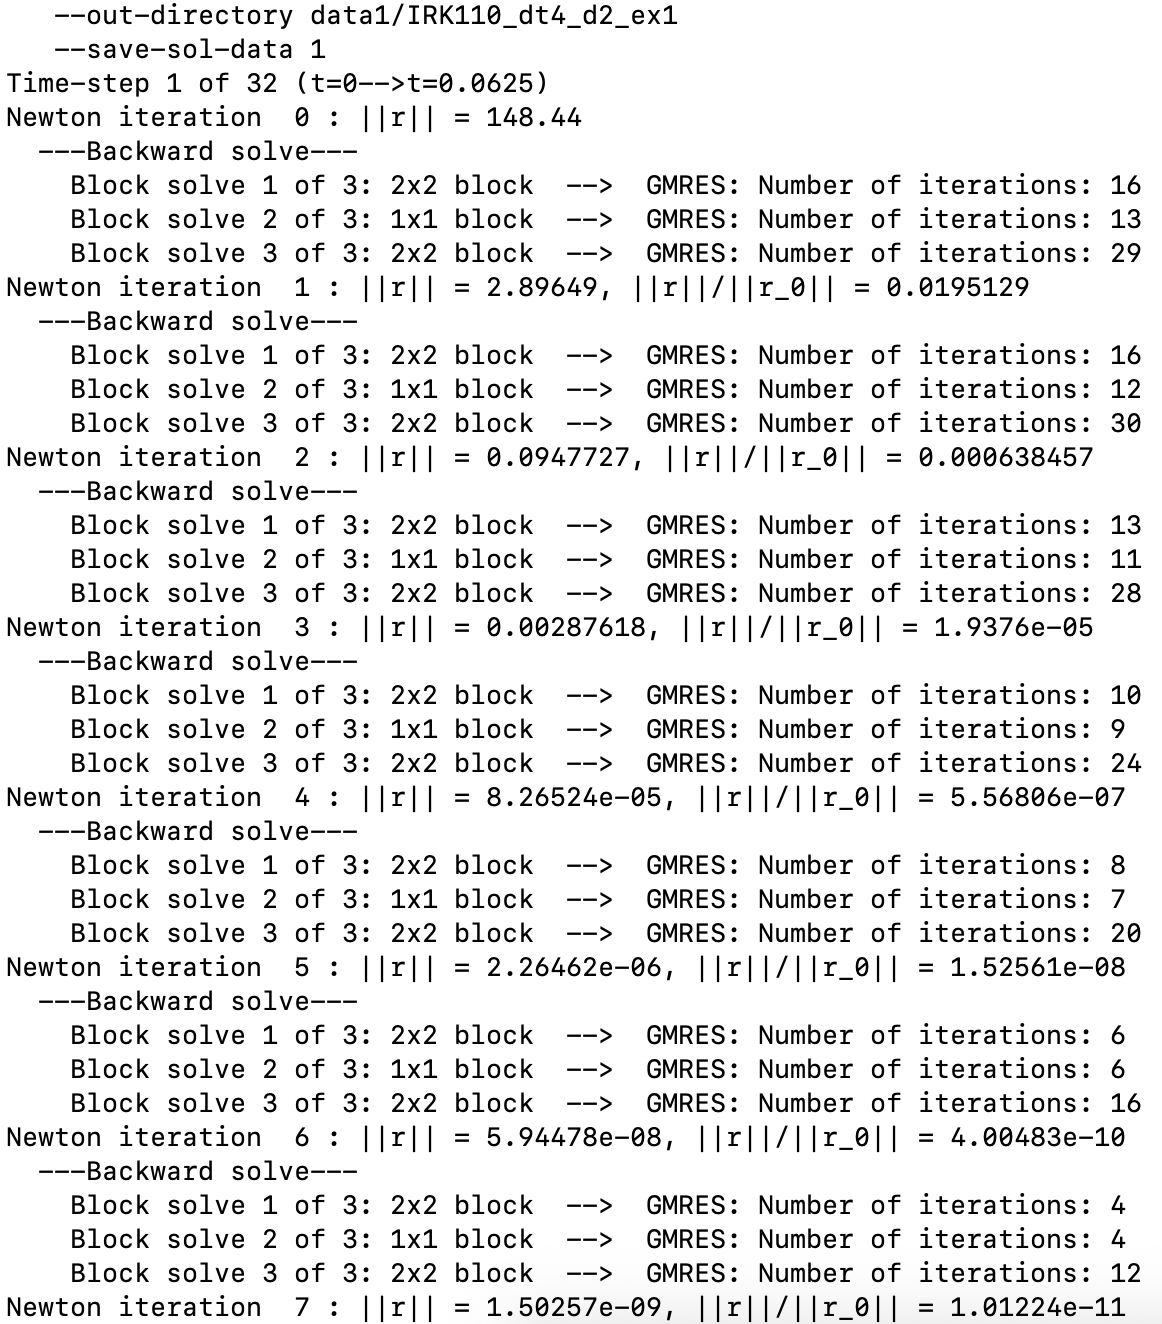
\includegraphics[width = 0.585\textwidth]{figures/simple_newton_basic}
\quad
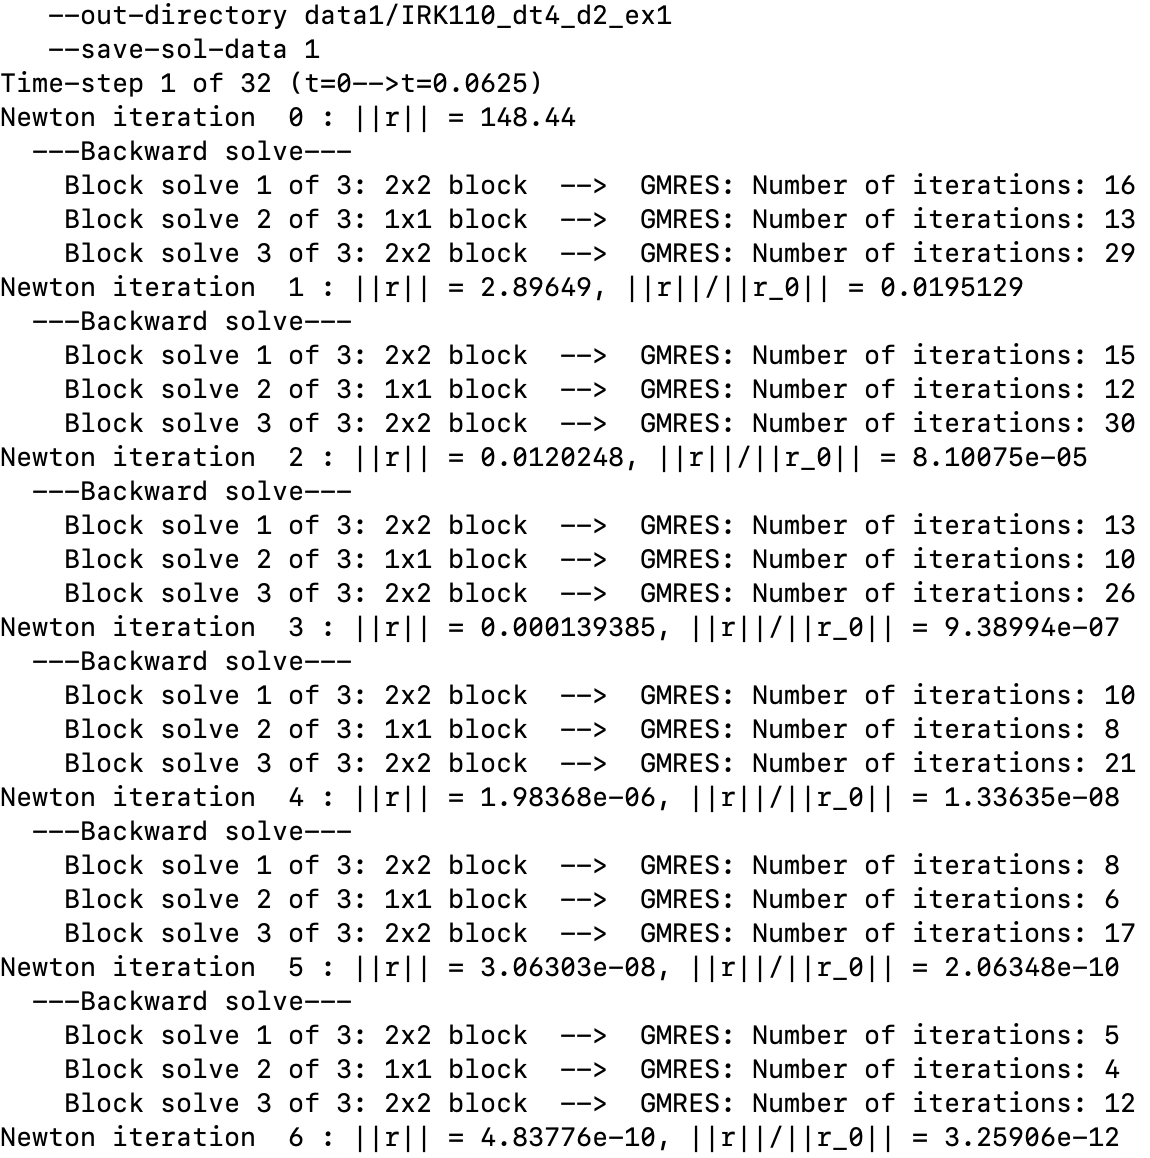
\includegraphics[width = 0.585\textwidth]{figures/simple_newton_better}
}
\caption{Simplified Newton convergence and that of its linear solver; first time step of finest resolution Gauss(10) solve from Figure \ref{fig:errors2D}.
\textbf{Left:} Jacobian fixed throughout Newton solve. \textbf{Right:} Updating approximate Jacobian each Newton iteration. Notice convergence on the \underline{right} is slightly faster.
\label{fig:simple_newton_convergence}
}
\end{figure}

\newpage
\section{Numerical results}

Numerically approximate the solution of the 2D nonlinear advection-diffusion problem,
\begin{align}
u_t + 0.85 u^2_x + 1.0 u^2_y = 0.3 u_{xx} + 0.25 u_{yy}  + s(x,y,t),
\quad (x,y,t) \in  (-1,1)^2 \times (0, 2)
\end{align}
Some remarks:
\begin{itemize}
\setlength\itemsep{0.5em}
\item Periodic spatial boundaries. All tests use 4 processors.

\item A $p$th-order IRK scheme is coupled with $p$th-order central finite differences in space (or $p$+1st-order if $p$ is odd, as for Lobatto IIIC and some SDIRK schemes).

\item Set $\delta t = 2 \delta x$

\item Tests in Figure \ref{fig:errors2D} indicate that the code is implemented and working properly since theoretically predicated convergence rates are obtained in all cases.

\item Solver settings:
\begin{itemize}
\setlength\itemsep{0.5em}
\item Newton: 
\begin{enumerate}
\item Approximate Jacobian updated at beginning of each time step
\item  \texttt{abs tol=rel tol=1e-10}
\end{enumerate}

\item GMRES: \texttt{abs tol=rel tol=1e-13}
\end{itemize}

These settings don't really make much sense because they lead to significant over-solving most of the time... E.g., really should be setting Newton tolerance proportionate to $\delta t^p$ and GMRES tolerances adaptively set within Newton iteration to reflect the size of the nonlinear residual and the convergence rate of Newton.

\item In terms of work done per accuracy, it seems like Gauss schemes are best, and Radau IIA schemes come in a close second, and that Lobatto IIIC schemes aren't even close. See Figure \ref{fig:iters2D}. But, I'm not quite sure how much to take away from this plot because tolerances are not set up very well...

\item 4th-order SDIRK schemes:
\begin{itemize}
\setlength\itemsep{0.5em}
\item A-stable: 3-stages, the diagonal entries on the upper triangular Schur matrix are $R_{ii} \approx 1.07$ (we solve linear systems like $R_{ii} I - \delta t {\cal N}'$)

\item L-stable: 5-stages, the diagonal entries on the upper triangular Schur matrix are $R(i,i)_{ii} \approx 4$. So the linear systems here have a larger identity perturbation c.f. the A-stable scheme, which is why they are easier to solve (they require fewer AMG iterations). 
\end{itemize}

\end{itemize}



\begin{figure}[H]
\centerline{
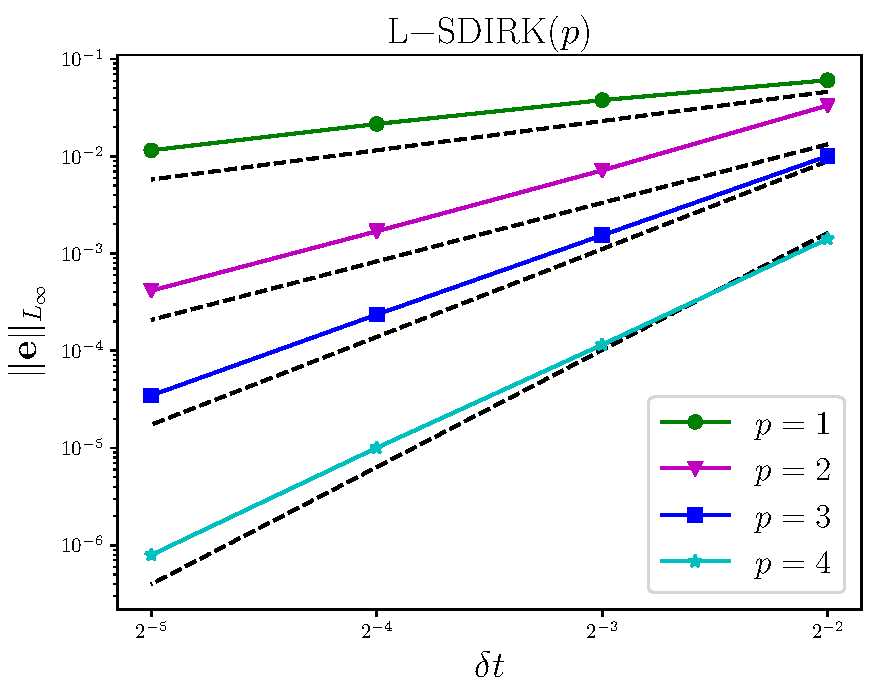
\includegraphics[width = 0.575\textwidth]{figures/LSDIRK_d2_ex1}
\quad
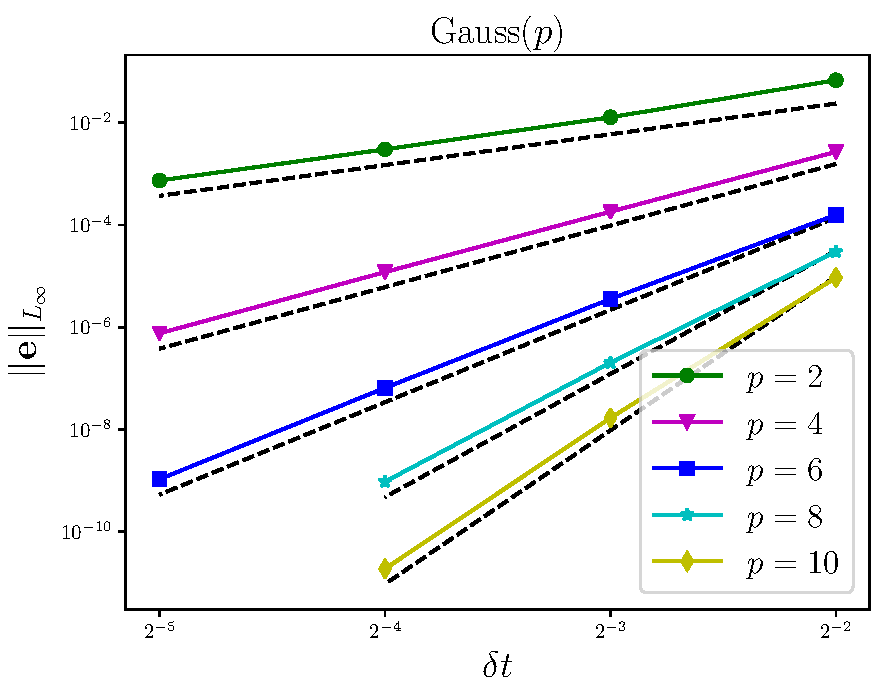
\includegraphics[width = 0.575\textwidth]{figures/Gauss_d2_ex1}
}
\centerline{
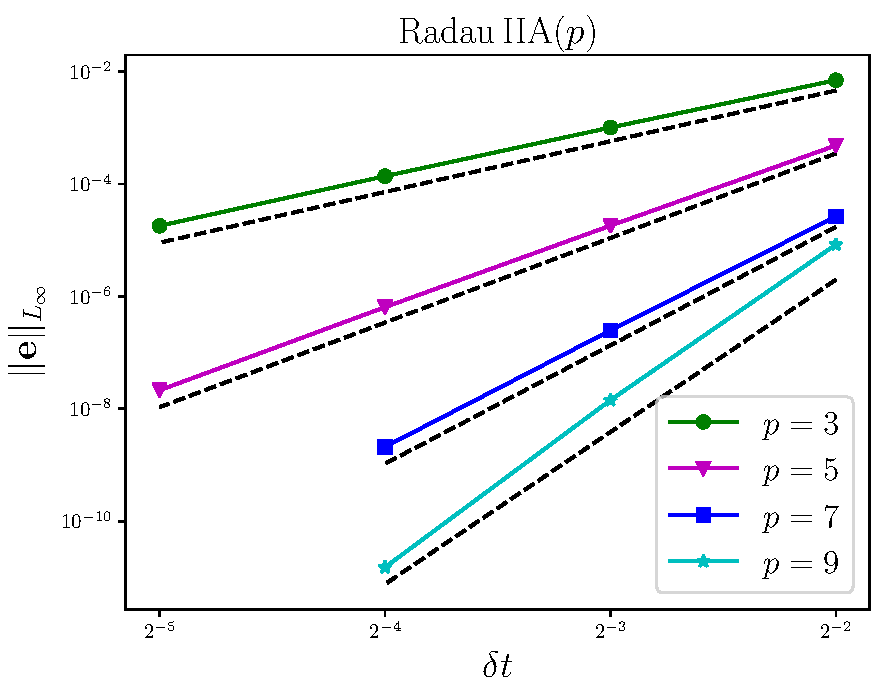
\includegraphics[width = 0.575\textwidth]{figures/RadauIIA_d2_ex1}
\quad
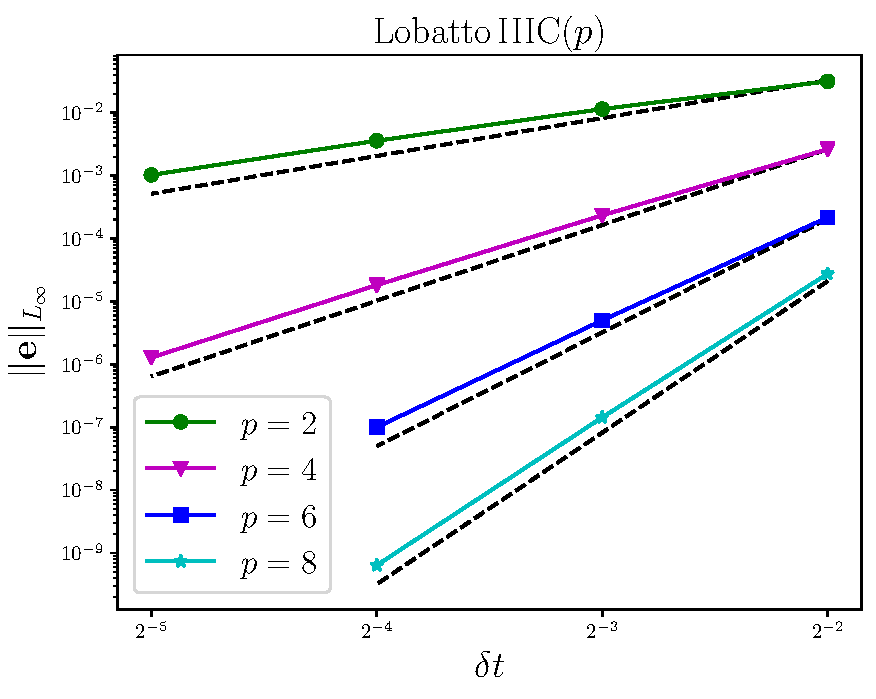
\includegraphics[width = 0.575\textwidth]{figures/LobattoIIIC_d2_ex1}
}
\caption{$L_{\infty}$ errors measured at $t \approx 2$. Theoretically predicted convergence rates of ${\cal O}(p)$ are shown as dashed black lines. ${\cal O}(p)$ IRK schemes are paired with ${\cal O}(p)$ spatial discretizations (or ${\cal O}(p+1)$ if $p$ is odd), and $\delta t = 2 \delta x$. 
\label{fig:errors2D}
}
\end{figure}


\begin{figure}[H]
\centerline{
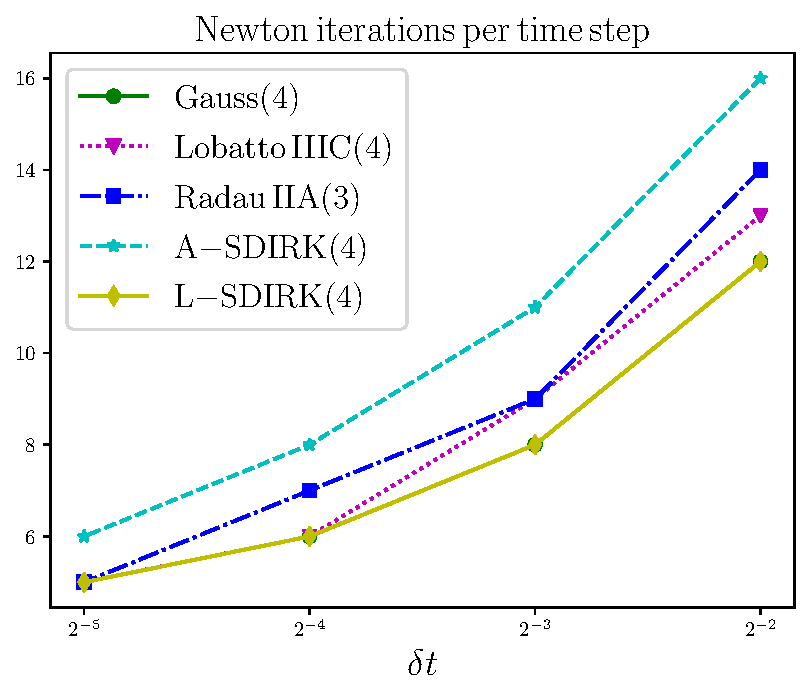
\includegraphics[width = 0.575\textwidth]{figures/newton_iters_O4_dim2}
\quad
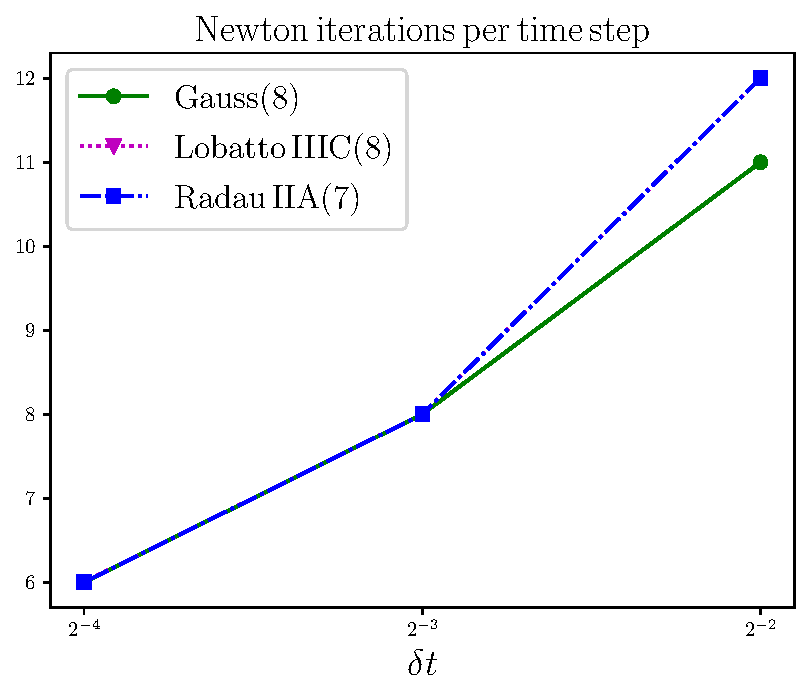
\includegraphics[width = 0.575\textwidth]{figures/newton_iters_O7_dim2}
}
\centerline{
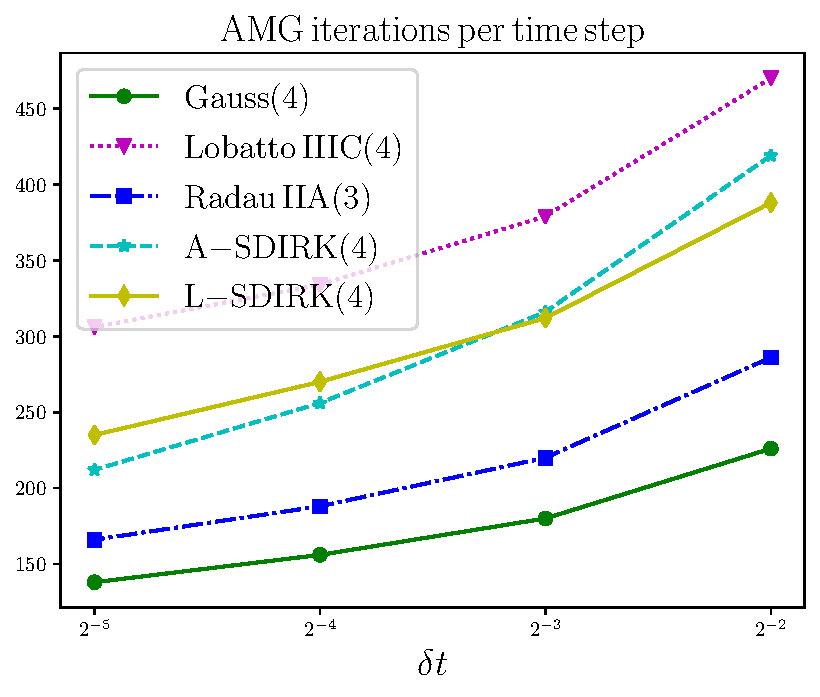
\includegraphics[width = 0.575\textwidth]{figures/amg_iters_O4_dim2}
\quad
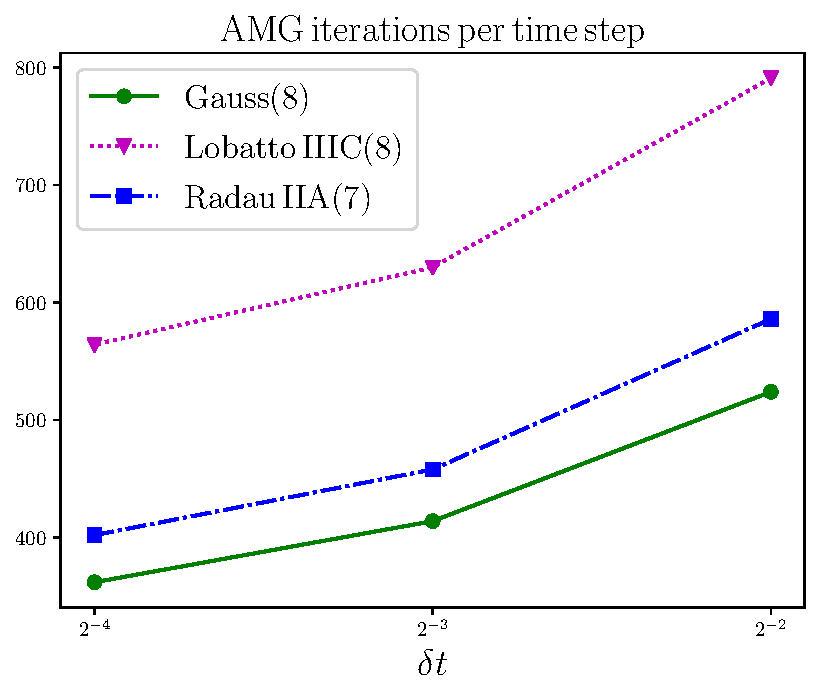
\includegraphics[width = 0.575\textwidth]{figures/amg_iters_O7_dim2}
}
\centerline{
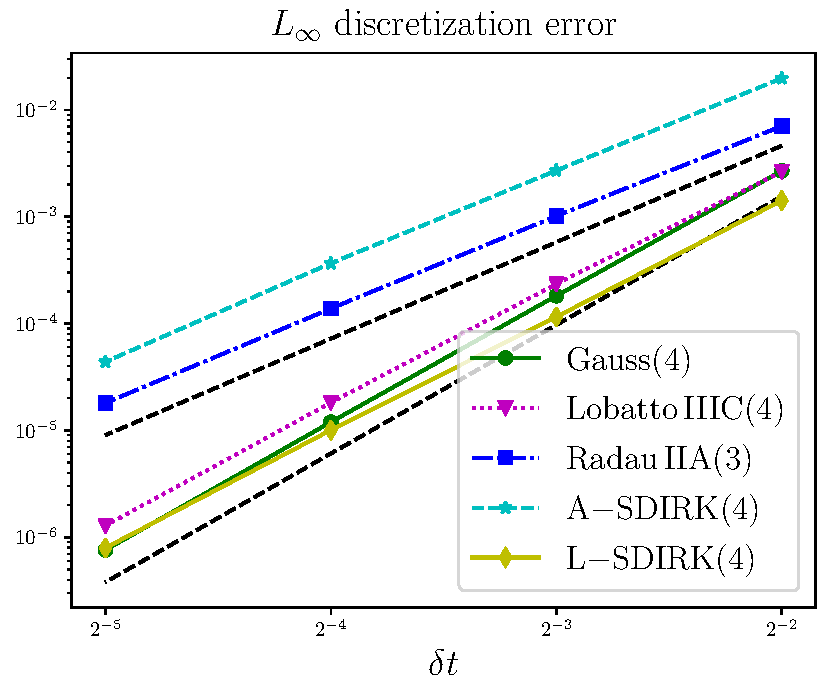
\includegraphics[width = 0.575\textwidth]{figures/errors_O4_dim2}
\quad
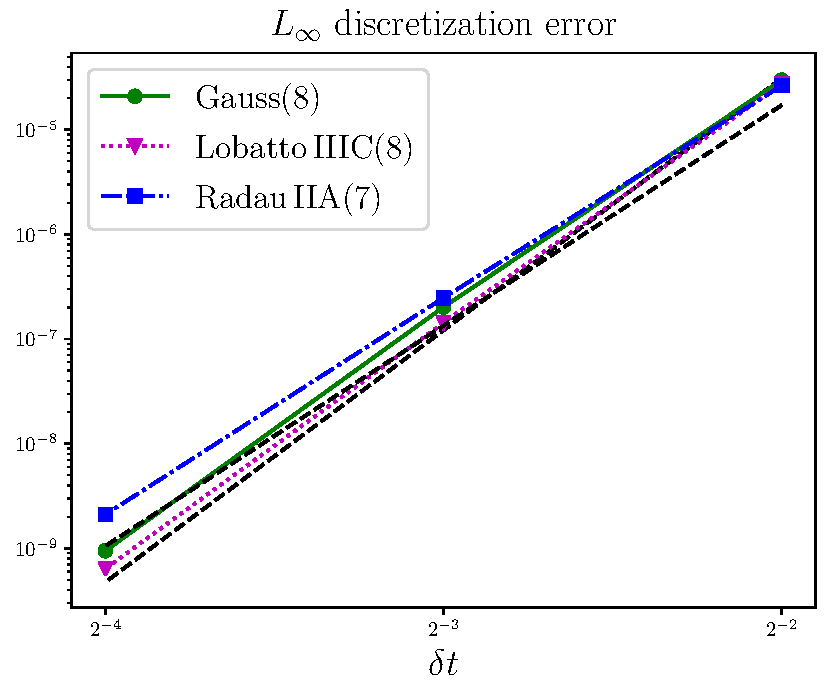
\includegraphics[width = 0.575\textwidth]{figures/errors_O7_dim2}
}
\caption{Average iterations per time step (data associated with convergence plots in Figure \ref{fig:errors2D}). \textbf{Left:} 4th(ish)-order schemes. \textbf{Right:} 8th(ish)-order schemes. \textbf{Top:} Newton iterations. \textbf{Middle:} AMG iterations. \textbf{Bottom:} Discretization errors. The systems that AMG is applied to have dimension $n = (16^2, 32^2, 64^2, 128^2)$ for $\delta t = (2^{-2}, 2^{-3}, 2^{-4}, 2^{-5})$. \tcp{Not really sure why so many Newton iterations decrease with resolution... See also Figure \ref{fig:iters1D}.}. In terms of work done per accuracy, it seems Gauss $<$ Radau IIA $\ll$ Lobatto IIIC. Note also for this particular problem, 4th-order Gauss does significantly better than both L-stable and A-stable 4th-order SDIRK schemes. Notice that the error constant for A-SDIRK(4) is much larger, and convergence appears only $\approx$3rd-order (Figure \ref{fig:iters1D} shows that eventually it does reach 4th-order however).
\label{fig:iters2D}
}
\end{figure}


\begin{figure}[H]
\centerline{
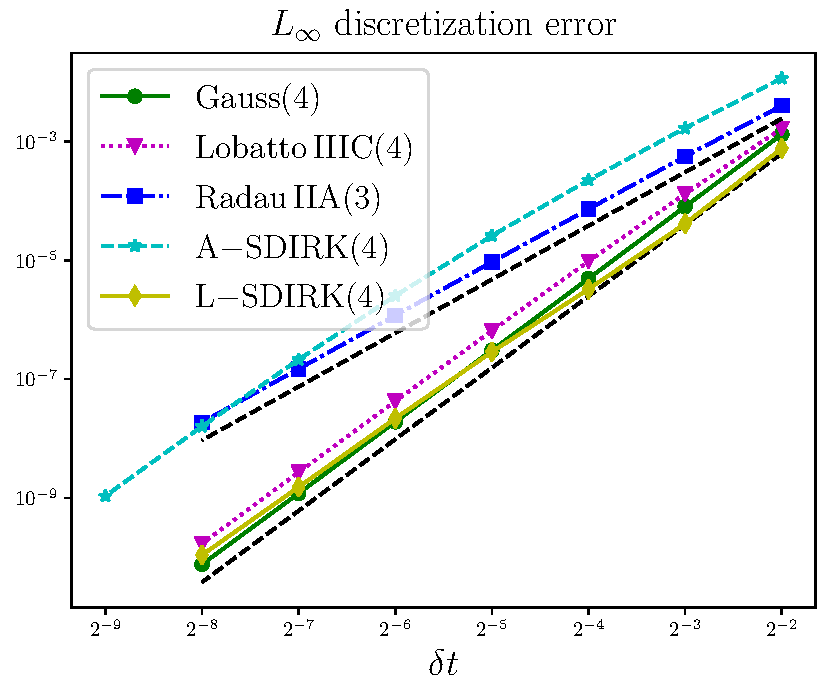
\includegraphics[width = 0.625\textwidth]{figures/errors_O4_dim1}
}
\centerline{
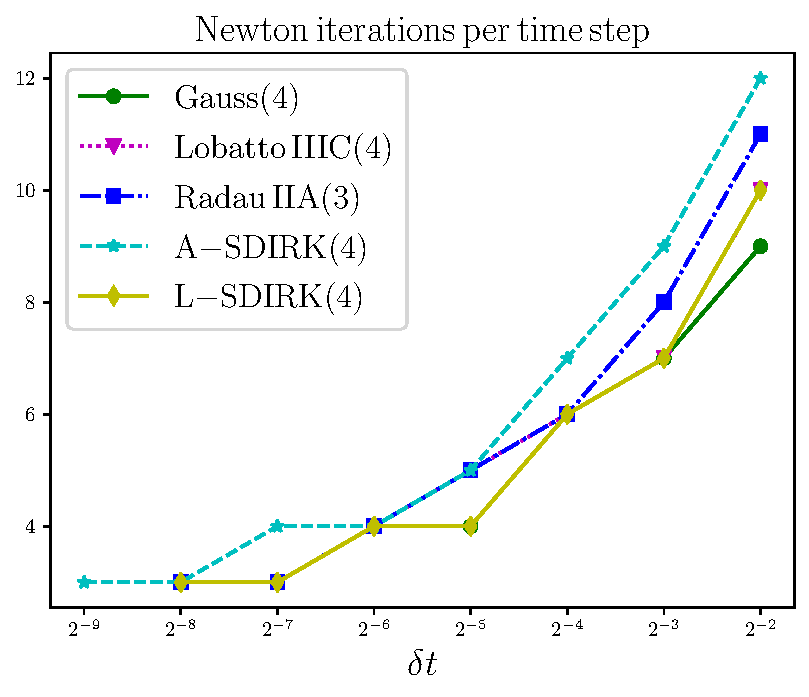
\includegraphics[width = 0.575\textwidth]{figures/newton_iters_O4_dim1}
\quad
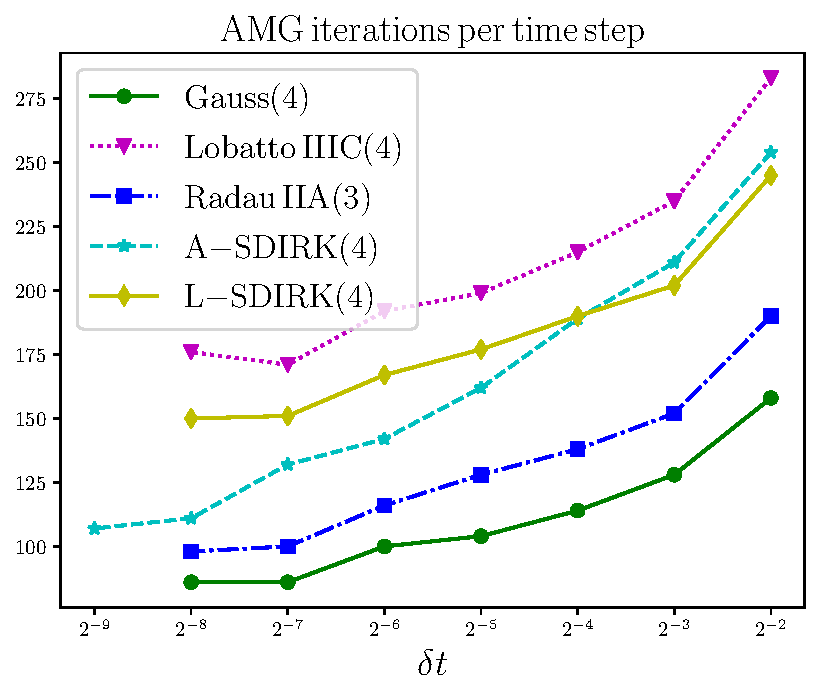
\includegraphics[width = 0.575\textwidth]{figures/amg_iters_O4_dim1}
}
\caption{Average iterations per time step for 4th(ish)-order discretizations of the \textbf{1D problem}, $u_t + 0.85 u^2_x = 0.3u_{xx} + s(x,t)$. Notice that A-SDIRK(4) does appear to eventually achieve 4th-order convergence, but the error is significantly larger than that of the other 4th-order schemes. Thus, Gauss(4) outperforms A-SDIRK(4) in terms of AMG iterations per accuracy.
\label{fig:iters1D}
}
\end{figure}


\section{A quasi-Newton algorithm}
The real Jacobian is
\begin{align}
F'(\bm{w}) &= A_0^{-1} \otimes M - 
\delta t
\begin{bmatrix} {\cal N}'_1 \\ 
& \ddots \\ 
& & {\cal N}'_s
\end{bmatrix}
\end{align}
where
\begin{align}
{\cal N}'_i \equiv {\cal N}' \left(\bm{u}_n + \delta t \bm{w}_i^0, t_n + c_i \delta t \right).
\end{align}
Before inverting the Jacobian, we scale it by $(Q_0^\top \otimes  I)$ from the left and $(Q_0 \otimes  I)$ from the right, making use of the Schur decomposition of $A^{-1}_0 = Q_0  R_0 Q^{\top}_0$,
\begin{align}
\widehat{F}'(\bm{w}) 
&\coloneqq (Q_0^\top \otimes  I) F'(\bm{w}) (Q_0 \otimes  I), \\
&= R_0 \otimes M - \delta t (Q_0^\top \otimes  I) \begin{bmatrix} {\cal N}'_1 \\ 
& \ddots \\ 
& & {\cal N}'_s
\end{bmatrix} (Q_0 \otimes I).
\end{align}
Now we write the second matrix in the form 
\begin{align}
\widehat{P} \coloneqq (Q_0^\top \otimes  I) \begin{bmatrix} {\cal N}'_1 \\ 
& \ddots \\ 
& & {\cal N}'_s
\end{bmatrix} (Q_0 \otimes I) 
=
\begin{bmatrix}
\bm{z}^\top_{1,1} \bm{{\cal N}}' & \cdots & \bm{z}^\top_{1,s} \bm{{\cal N}}' \\
\vdots & & \vdots \\
\bm{z}^\top_{s,1} \bm{{\cal N}}' & \cdots & \bm{z}^\top_{s,s} \bm{{\cal N}}'
\end{bmatrix},
\end{align}
where $\bm{z}^\top_{k,\ell} = \Big((Q_0^\top)_{k ,1} (Q_0)_{1, \ell}, \ldots, (Q_0^\top)_{k, s} (Q_0)_{s, \ell} \Big) \in \mathbb{R}^s$ is a row vector, and $\bm{{\cal N}}' = ({\cal N}'_1, \ldots, {\cal N}'_s)$ is a column vector of the Jacobians of ${\cal N}_i$, meaning that
\begin{align}
\bm{z}^\top_{k,\ell} \bm{{\cal N}}' = \sum \limits_{i = 1}^s (z_{k, \ell})_i {\cal N}'_i.
\end{align}
Note that by the orthogonality of $Q_0$,
\begin{align}
\bm{z}^\top_{k,\ell} \bm{1} 
= 
(Q_0^\top Q_0)_{k, \ell}
=
\begin{cases}
1, \quad k = \ell,\\
0, \quad k \neq \ell,
\end{cases}
\end{align}
which tends to suggest that the block diagonal entries of $P$ are most important \tcp{(e.g., think about the case in which the matrices in $\bm{{\cal N}}'$ approximately have the same eigenvectors and eigenvalues)}. 

In the quasi-Newton algorithm, we choose some \underline{block upper triangular} $\widetilde{P} \approx \widehat{P}$, which has a (block) sparsity pattern contained within that of $R_0 \otimes M$. The point of making it block upper triangular is that we can invert \textit{exactly} the resulting approximate Jacobian via back substitution. So, during the Newton solves we ``exactly'' invert the approximate Jacobian, 
\begin{align}
\widetilde{F}'(\bm{w}) 
\coloneqq  
R_0 \otimes M - 
\delta t \tilde{P}
\approx
R_0 \otimes M - 
\delta t P
\eqqcolon
\widehat{F}'(\bm{w}).
\end{align}

There are a few different options for choosing $\widetilde{P} \approx \widehat{P}$:
\begin{enumerate}
\setlength\itemsep{0.5em}

\item[0.] \textbf{(biggest approximation)} Truncate $\widehat{P}$ to be block diagonal and them lump the coefficients of $\bm{z}_{ii}$ to the largest one so that each diagonal block of $\widetilde{P}$ contains only one matrix from $\bm{{\cal N}}'$.

\item[1.] \textbf{(medium approximation)} Truncate $\widehat{P}$ to be block diagonal (can include the off-diagonal entries in $2 \times 2$ diagonal blocks, or not)

\item[2.] \textbf{(smallest approximation)} Truncate $\widehat{P}$ to be block upper triangular. This means doing a lot of matrix-vector products (just how much work this is depends on the implementation, I think; can maybe try and exploit the underlying Kronecker-product structure to reduce this), but potentially improving convergence of Newton's method

\end{enumerate}

\subsection{Numerical results}

Am having trouble coming up with a good test problem... Struggling to find a meaningful nonlinear, diffusion-dominated PDE?
\begin{itemize}
\setlength\itemsep{0.5em}

\item Current problem from previous example is no good because as mesh is refined, discrete diffusion $\gg$ discrete advection, so problem looks more and more linear (this is why in Figure \ref{fig:iters2D} and \ref{fig:iters1D} the Newton iterations approach 1 as the spatial/temporal mesh is refined). 

\item Also, for a fixed mesh resolution, as I time step, the number of Newton iterations per time step decreases. \tcp{Why?!} This makes it too hard to make comparisons

\end{itemize}

\vspace{1cm}
So... as an initial test, measure number of iterations for one time step ($t = 0 \to 0.3125$) of 
\begin{align}
u_t + 0.85 u^2_x + 1.0 u^2_y = 0.3 u_{xx} + 0.25 u_{yy}  + s(x,y,t),
\end{align}
using \tcp{$\delta t = 10 \delta x$} (this makes problem much harder for Newton, and highlights differences between simple- and quasi-Newton solvers), and $n_x \times n_y = 64 \times 64$ (4096 spatial DOFs). See Table \ref{tb:iters}.


\begin{table}[tbhp] 
\caption{
Number of Newton and AMG iterations. ``Simple'' = simplified Newton, ``Quasi(0),(1),(2)'' = quasi Newton with different approximations $\widetilde{P}$ with increasing cost per Newton iteration. \tcp{Interpret results with a grain of salt because there are hidden costs for the different Newton methods including matrix-vector products, assembling of Jacobians, assembling of AMG preconditioners.} 
\label{tb:iters}
}
\begin{center}
\begin{tabular}{|c V{3} cccc|} 
\hline
&
\multicolumn{4}{c|}{\textbf{Newton iterations}/AMG iterations} 
\\
\hline
Discretization
&
Simple
& 
Quasi(0)
&
Quasi(1)
&
Quasi(2)
\\
\Xhline{2\arrayrulewidth} 
ASDIRK(4)+C4 & \textbf{23}/519 & \textbf{4}/118 & \textbf{4}/118 & \textbf{4}/118 \\
\hline
LSDIRK(4)+C4 & \textbf{19}/570 & \textbf{4}/169 & \textbf{4}/169 & \textbf{4}/169 \\
\hline
Gauss(4)+C4 & \textbf{17}/322 & \textbf{4}/92  & \textbf{4}/92  & \textbf{4}/92  \\
\hline 
Radau IIA(5)+C4 & \textbf{19}/646 & \textbf{9}/330 & \textbf{9}/329 & \textbf{6}/249\\
\hline 
\hline
Gauss(6)+C6 & \textbf{17}/531 & \textbf{8}/277 & \textbf{8}/278 & \textbf{7}/250\\
\hline 
Lob IIIC(6)+C6 & \textbf{19}/927 & \textbf{13}/712 & \textbf{11}/620 & \textbf{7}/436 \\
\hline
Radau IIA(7)+C6 & \textbf{18}/868 & \textbf{9}/464 & \textbf{9}/462 & \textbf{7}/386 \\
\hline 
\hline
Gauss 8(8)+C8 & \textbf{17}/794 & \textbf{8}/434 & \textbf{8}/434 & \textbf{6}/364 \\
\hline 
Lob IIIC 8(8)+C8 & \textbf{18}/1211 & \textbf{13}/922 & \textbf{12}/817 & \textbf{9}/672 \\
\hline 
Radau IIA(9)+C8 & \textbf{17}/1090 & \textbf{9}/596 & \textbf{9}/582 & \textbf{7}/504 \\
\hline 
\end{tabular}
\end{center}
\end{table}

\begin{itemize}
\setlength\itemsep{0.5em}

\item Note SDIRK and Gauss(4) have sparse $Q_0$, so the different quasi-Newton variants are the same (hence constant Newton/AMG iterations)

\item Quasi-Newton converges significantly faster than Simple-Newton

\end{itemize}

\newpage
\subsection{Newer results}

\begin{table}[H] 
\caption{
Number of Newton and AMG iterations. ``Simple'' = simplified Newton, ``Quasi(0),(1),(2)'' = quasi Newton with different approximations $\widetilde{P}$ with increasing cost per Newton iteration \tcb{using larger time step $\delta t = 10 \times h$}.
\label{tb:iters_newer}
}
\begin{center}
\begin{tabular}{|c V{3} cccc|} 
\hline
&
\multicolumn{4}{c|}{\textbf{Newton iterations}/AMG iterations($\gamma = \eta$, $\gamma = \eta + \beta^2/\eta$)} 
\\
\hline
Discretization
&
Simple
& 
Quasi(0)
&
Quasi(1)
&
Quasi(2)
\\
\Xhline{2\arrayrulewidth} 
Gauss(4)+C4 & \textbf{17}/(296,268) & \textbf{4}/(84,76)  & --  & --  \\
\hline 
Lob IIIC(4)+C4 & \textbf{20}/(689,573) & \textbf{17}/(555,447) & \textbf{13}/(453,373) & \textbf{10}/(421,363)\\
\hline 
Radau IIA(5)+C4 & \textbf{19}/(604,490) & \textbf{9}/(300,246) & \textbf{9}/(296,244) & \textbf{6}/(244,208)\\
\hline 
\hline
Gauss 8(8)+C8 & \textbf{17}/(794,656) & \textbf{8}/(414,344) & \textbf{8}/(412,342) & \textbf{6}/(364,310) \\
\hline 
Lob IIIC 8(8)+C8 & \textbf{18}/(1211,957) & \textbf{13}/(880,706) & \textbf{12}/(803,645) & \textbf{9}/(672,550) \\
\hline 
Radau IIA(9)+C8 & \textbf{17}/(1090,844) & \textbf{9}/(589,465) & \textbf{9}/(578,458) & \textbf{7}/(504,412) \\
\hline 
\end{tabular}
\end{center}
\end{table}

\begin{table}[H] 
\caption{
Number of Newton and AMG iterations. ``Simple'' = simplified Newton, ``Quasi(0),(1),(2)'' = quasi Newton with different approximations $\widetilde{P}$ with increasing cost per Newton iteration \tcb{using smaller time step $\delta t = 1 \times h$}.
\label{tb:iters_newer2}
}
\begin{center}
\begin{tabular}{|c V{3} cccc|} 
\hline
&
\multicolumn{4}{c|}{\textbf{Newton iterations}/AMG iterations($\gamma = \eta$, $\gamma = \eta + \beta^2/\eta$)} 
\\
\hline
Discretization
&
Simple
& 
Quasi(0)
&
Quasi(1)
&
Quasi(2)
\\
\Xhline{2\arrayrulewidth} 
Gauss(4)+C4 & \textbf{5}/(104,84) & \textbf{3}/(68,54)  & --  & --  \\
\hline 
Lob IIIC(4)+C4 & \textbf{6}/(265,168) & \textbf{5}/(232,152) & \textbf{5}/(235,151) & \textbf{5}/(225,145)\\
\hline 
Radau IIA(5)+C4 & \textbf{5}/(199,139) & \textbf{4}/(165,114) & \textbf{4}/(165,114) & \textbf{4}/(169,116)\\
\hline 
\hline
Gauss 8(8)+C8 & \textbf{5}/(254,200) & \textbf{4}/(222,176) & \textbf{4}/(222,176) & \textbf{4}/(226,176) \\
\hline 
Lob IIIC 8(8)+C8 & \textbf{5}/(424,280) & \textbf{5}/(403,267) & \textbf{5}/(398,264) & \textbf{4}/(357,233) \\
\hline 
Radau IIA(9)+C8 & \textbf{5}/(365,261) & \textbf{4}/(301,215) & \textbf{4}/(301,215) & \textbf{4}/(299,219) \\
\hline 
\end{tabular}
\end{center}
\end{table}


\renewcommand{\tabcolsep}{4pt}
\renewcommand{\arraystretch}{1.15}
\begin{table}[!ht]
  \centering
  \begin{tabular}{| c | c | c |}  % chktex 44
  \hline
Method & &  \\ \hline
\multirow{ 3}{*}{Gauss(8)}
&$\beta^2/\eta^2$ & 1.59 / 0.09 \\
&$\gamma = \eta$  -- & 20 / 11\\
&$\gamma = \gamma_*$ & 13 / 11\\ \hline
\multirow{ 3}{*}{Radau IIA(9)}
&$\beta^2/\eta^2$ & 0 / 3.20 / 0.32	\\
&$\gamma = \eta$ &  8 / 24 / 13\\
&$\gamma = \gamma_*$ & 8 / 14/ 11 \\ \hline
\multirow{ 3}{*}{Lobatto IIIC(8)}
&$\beta^2/\eta^2$ & 0 / 4.88 / 0.38 \\
&$\gamma = \eta$ & 8 / 29 / 14\\
&$\gamma = \gamma_*$ & 8 / 15 / 12\\
  \hline
  \end{tabular}
  \caption{
Number of GMRES iterations for each stage when solving $u_t = \Delta u + s$, with a single time step of $\delta t = h = 1/256$. Different values of $\gamma$ are used in the preconditoner, as indicated.
}
\label{tab:cond_iters}
\end{table}

\end{document}


